\documentclass[tikz,border=10pt]{standalone}
\usepackage{pgfplots}
\usetikzlibrary{intersections, calc}

\begin{document}
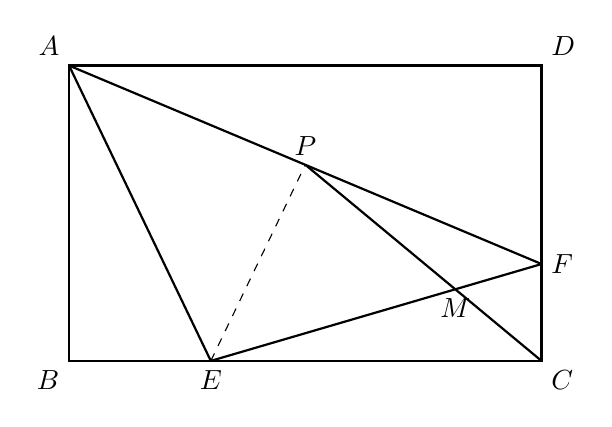
\begin{tikzpicture}[
    scale=1.5, 
    important line/.style={thick},
    dashed line/.style={dashed, thin},
    every node/.style={color=black}
]

    % 1. 定义矩形的四个顶点坐标
    % 设定宽度为4，高度为2.5
    \coordinate (A) at (0, 2.5);
    \coordinate (B) at (0, 0);
    \coordinate (C) at (4, 0);
    \coordinate (D) at (4, 2.5);

    % 2. 绘制矩形边界
    \draw[important line] (A) -- (B) -- (C) -- (D) -- cycle;

    % 3. 定义点 E (在 BC 上) 和 点 F (在 CD 上)
    \coordinate (E) at (1.2, 0); % E靠近B点
    \coordinate (F) at (4, 0.82); % F在CD中间偏下

    % 4. 绘制线段 AE, AF, EF (形成的三角形 AEF)
    \draw[important line] (A) -- (E);
    \draw[important line, name path=lineAF] (A) -- (F);
    \draw[important line, name path=lineEF] (E) -- (F);

    % 5. 定义点 P 并连接 PC
    % P点位于 AF 上，根据原图估算位置
    \coordinate (P) at ($(A)!0.5!(F)$); 
    \draw[important line, name path=linePC] (P) -- (C);

    % 6. 计算交点 M 并绘制辅助虚线 EP
    % 计算 PC 与 EF 的交点
    \fill [name intersections={of=linePC and lineEF, by=M}];
    \draw[dashed line] (E) -- (P);

    % 7. 标注所有点的标签
    \node[above left]  at (A) {$A$};
    \node[below left]  at (B) {$B$};
    \node[below right] at (C) {$C$};
    \node[above right] at (D) {$D$};
    \node[below]       at (E) {$E$};
    \node[right]       at (F) {$F$};
    \node[above]       at (P) {$P$};
    \node[below]       at (M) {$M$};

\end{tikzpicture}
\end{document}